\section{Introduction}
\label{sec:intro}

Although the human nervous system is very different from a cockroach’s, the structure and function of our individual neurons is actually very similar. This similarity allows us to learn about the human brain by studying cockroaches'. Invertebrates, including insects like cockroaches, are important model systems in neurophysiology because of their small, manageable size, the ability to easily access specific motor neurons that innervate entire specific muscle groups, and the presence of central pattern generators (CPG) that produce locomotive behaviors. They provide a convenient target for invasive procedures that would not be attempted in vertebrate animals. Finally, the ability to switch CPGs on or off, or to drive a particular function (motor, brake, spring) on a limb with a single motor neuron, make them a tractable system with which to attempt closed loop control. 
%Hollywood attention grabber.
\begin{figure}[ht!]
\centering
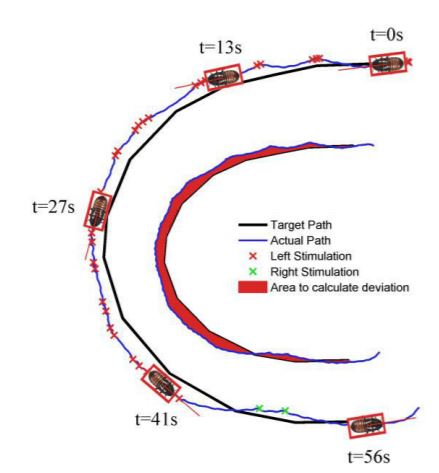
\includegraphics[scale=0.5]{Figures/motivation1.JPG}
\caption{A future goal is to steer a RoboRoach under active neural control, from \citep{whitmire2013kinect}}
\label{fig:motivation1}
\end{figure}

\begin{figure}[ht!]
\centering
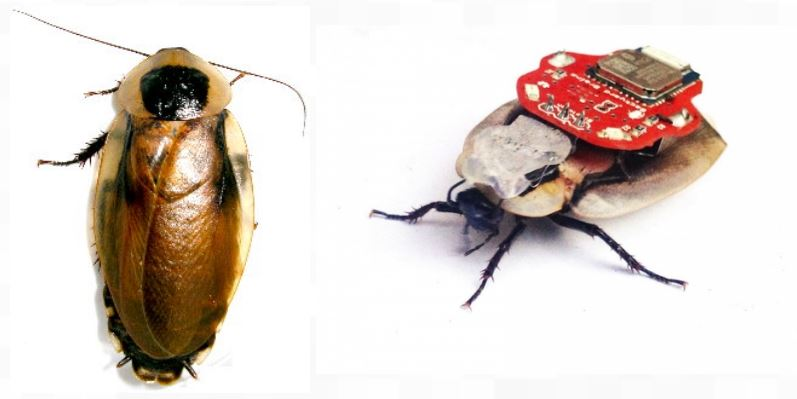
\includegraphics[scale=0.5]{Figures/motivation2.JPG}
\caption{Transformation from cockroach to RoboRoach, from \citep{backyardbrains2020roboroach}}
\label{fig:motivation2}
\end{figure}


% Literature Review
\subsection{Steering insects via electrical stimulation}
Steering of insects using electrical stimulation is an active area of research. \citet{moore1998directed} were able to ``drive'' cockroaches through a zig-zagged track. They found that, although results varied, only a small fraction of the cockroaches responded and were consistently sensitive to the stimuli \citep{moore1998directed}. They also discovered that, in most cases, current directed toward the base of an antenna resulted in faster forward motion whereas current directed further down the antenna resulted in slow walking, halting, and even reverse motion \citep{moore1998directed}.

A more detailed study of higher neural structures showed that the central complex, a part of the arthropod brain that receives sensory information and outputs to premotor regions, supervises locomotion \citep{guo2013neural}. \citet{guo2013neural} performed the same type of experiment as \citet{moore1998directed}, but also created firing maps based on the roaches' continuously changing speed and direction, which demonstrated that many of the central complex units they recorded were tuned to particular turning and forward walking speeds.

Like the previous two experiments, \citet{holzer1997locomotion} also applied electrical stimulation of nerves using an electronic backpack. Unlike the previous experiments, however, they recorded their measurements on a styrofoam trackball connected to a computer, which allowed them to record the turning rate and forward movement in response to stimulation to the roach's antennae \citep{holzer1997locomotion}. Their experiments also showed that, despite large variance, they could achieve directional locomotion control by stimulating the nerves of cockroaches' antennae.

\citet{whitmire2013kinect} demonstrated how engineering can be used to steer cockroaches by adding external computer vision, making the application of electrical stimulus autonomous. By observing successful trials of cockroach steering, the team found that the deviation from the prescribed path and the net angular change and velocity when turning could be used to create a quantitative analysis of the experiment \citep{whitmire2013kinect}. Unlike the previous study, which required a human operator to manually stimulate with a remote control, this one steered the roaches using a computer vision platform that automatically stimulates the roaches \citep{whitmire2013kinect}. The computer vision platform allowed for automated variation in stimulation patterns as the cockroach adjusted its path \citep{whitmire2013kinect}. From the quantitative analysis, the team was able to get a precise estimate of the effects of each stimulus, allowing the to optimize the efficacy of their stimulation technique \citep{whitmire2013kinect}. 





\subsection{Antennae as targets for electrical stimulation}
In studies of antenna mechanics, locomotion, and the environment, \citet{Mongeau2014} observed high-speed navigation in cockroaches and found that, when the tip of the antenna is projected backward, the roach maintains greater body-to-wall distance with fewer body collisions and less leg–wall contact than when the tip is projecting forward. The team then hypothesized that the mechanosensory hairs at the tip of the antenna determine a moving cockroach's behavior with a wall \citep{Mongeau2014}. To test their hypothesis, \citet{Mongeau2014} performed laser ablation of chemo-mechanosensory hairs and added artificial hairs to a robotic antenna. The team found that in both the natural and artificial systems, the presence of hairs categorically increased an antenna’s probability of switching state \citep{Mongeau2014}. Antenna hairs, once thought to only play a role in sensing, are sufficient for (passively) mechanically reconfiguring the state of the entire antenna when coupled with forward motion \citep{Mongeau2014}. The results of this study are useful to my study because they demonstrate the effect of the presence of hairs on the antenna on the movement and navigation of the cockroach. Furthermore, stimulation of these hairs could have an effect on the forward or backward motion of the roach.

While cockroaches are a model organism for polypedal terrestrial locomotion, hawkmoths (\emph{Manduca sexta}) are often used in aerial studies due to the relative ease in acquiring them and their manageable size for probing with electrodes.  Their large antennae are a major sensor used in flight control \citep{antennal}.  \citet{wireless} used a radio controlled, programmable, miniature stimulator and demonstrated that ultra-low-current electrical stimulation of antennal muscles in freely-flying hawkmoths allowed them to achieve some flight control over the moths. The mechanosensors at the base of the antennae mediate an abdominal flexion response to rotations that can be employed in steering \citep{wireless}. By electrically stimulating the antennae of hawkmoths, the team was able to observe repeatable, transient changes in the animals’ pitch angle, as well as less predictable changes in flight speed and flight altitude \citep{wireless}. \citet{antennal} demonstrated that the mechanosensors in the bases of the antennae are necessary for flight stability in hawkmoths. Both of these studies provide insight into how and where electrical stimulation of the antenna could affect directional control over cockroaches.

Antennae are not the only sensor pathway that could be co-opted to actively control an insect. In dipteran flies, the second pair of wings is modified to become an inertial sensor called a haltere.  The halteres are evolutionarily derived from wings and the two possess the same sensory structures, campaniform sensilla \citep{Dickerson2014}. \citet{Dickerson2014} attached magnets to the wings of moths and simulated pitch stimulus via a rotating magnetic field during tethered flight, and found that they elicited the same vertical abdominal flexion reflex these animals exhibit in response to visual or inertial pitch stimuli. Their results indicated that insect wings serve as both actuators and sensors that initiate reflexes that control body dynamics \citep{Dickerson2014}.

\subsection{Alternatives to direct neural control via stimulation}
Cyborg insects are not the only ways that humans study and exploit animal behavior to achieve useful tasks. One team developed a a mobile robot that could enter a circular arena, gather a flock of ducks and maneuver them safely to a specified goal position \citep{robot}. The team started by creating a basic model of duck flocking behavior and a subsequent simulation to guide a flock-control algorithm design \citep{robot}. They used this simulation to test their design, and then transferred their design into a physical robot that successfully achieved the same results with real ducks\citep{robot}.

\citet{Butler2005} addressed the problem of herding and how labor intensive it is to herd livestock over large paddocks while the animals are rotated frequently to achieve pasture management constraints. Not only that, but herding is physically hard work, often carried out in extreme weather conditions and remote locations \citep{Butler2005}. To solve the problem, the team introduced the concept of a virtual fence, a position-aware computer collar device which applies a stimulus to an animal as a function of its pose with respect to the fence lines \citep{Butler2005}. The team used sound stimuli as opposed to an electrical shock \citep{Butler2005}. This study is particularly interesting because the team successfully stimulated a change in behavior in the cows without using an electrical stimulus. The cows' reaction may have been different if the team had used electric stimulus instead of sound. In trying to achieve both position and speed control in my study, I may experiment with types of stimulation other than current to the antenna.





\subsection{Research goals}
Based on the findings of these previous experiments, I intend to replicate their experiments to evaluate the feasibility of a future lab exercise involving cyborg cockroaches. My ultimate aim of steering a cockroach is to learn about neurophysiological and neuromechanical principles which may be applicable in restoring human function. 

I hypothesize that modulating current to the antennae will modulate speed. If locomotion is dependent on the action of several central pattern generators being excited or inhibited, there may be limited effects on turning at the antennae and I may have to stimulate some other location to alter speed. 
Candidates for other places to stimulate are the cerci and central complex within the brain. From an engineering perspective, I want to be able to control the speed and direction of a robot. Since the previous studies have demonstrated success in direction control, my objective will be to add speed control.







